%!TEX TS-program = xelatex
\documentclass[xetex,10pt,aspectratio=43]{beamer} 
%设置为 Beamer 文档类型,设置字体为 10pt,长宽比为16:9,数学字体为 serif 风格
\batchmode

\usefonttheme{professionalfonts}
\usetheme{Berlin} %主题
\usecolortheme{sustech} %主题颜色

\usepackage[UTF8]{ctex}
\usepackage{unicode-math}
\usepackage{graphicx}
\usepackage{animate}
\usepackage{tikz}
\usepackage{hyperref}

%导入一些用到的宏包
\usepackage{amsmath,bm,amssymb,enumerate,epsfig,bbm,calc,color,ifthen,capt-of,multimedia}
\usepackage[ruled,linesnumbered]{algorithm2e}

\usepackage{fancybox}
\usepackage{xcolor}
\usepackage{times}
\usepackage{listings}

\usepackage{booktabs}
\usepackage{colortbl}

\newcommand{\Console}{Console}
\lstset{ %
	backgroundcolor=\color{white},   % choose the background color
	basicstyle=\footnotesize\rmfamily,     % size of fonts used for the code
	columns=fullflexible,
	breaklines=true,                 % automatic line breaking only at whitespace
	captionpos=b,                    % sets the caption-position to bottom
	tabsize=4,
	commentstyle=\color{mygreen},    % comment style
	escapeinside={\%*}{*)},          % if you want to add LaTeX within your code
	keywordstyle=\color{blue},       % keyword style
	stringstyle=\color{mymauve}\ttfamily,     % string literal style
	numbers=left, 
	%	frame=single,
	rulesepcolor=\color{red!20!green!20!blue!20},
	% identifierstyle=\color{red},
	language=c
}

\setmathfont{XITS Math}

\definecolor{mygreen}{rgb}{0,0.6,0}
\definecolor{mymauve}{rgb}{0.58,0,0.82}
\definecolor{mygray}{gray}{.9}
\definecolor{mypink}{rgb}{.99,.91,.95}
\definecolor{mycyan}{cmyk}{.3,0,0,0}

%题目,作者,学校,日期
\title{离散数学基础}
\subtitle{\fontsize{9pt}{14pt}\textbf{集合的基本概念}}
\author{中山大学MOOC课程组}
\institute{\fontsize{8pt}{14pt}中山大学计算机学院}
\date{\today}

%学校Logo
%\pgfdeclareimage[height=0.5cm]{sustech-logo}{sustech-logo.pdf}
%\logo{\pgfuseimage{sustech-logo}\hspace*{0.3cm}}

\AtBeginSection[]
{
	\begin{frame}<beamer>
		\frametitle{\textbf{目录}}
		\tableofcontents[currentsection]
	\end{frame}
}
\beamerdefaultoverlayspecification{<+->}

%图片
\graphicspath{{img/}}
% -----------------------------------------------------------------------------
\begin{document}
	% -----------------------------------------------------------------------------
	
	\frame{\titlepage}
	
	\section[目录]{}   %目录
	\begin{frame}{目录}
		\tableofcontents
	\end{frame}

	\section{基本知识回顾}
	
	\subsection{集合的基本术语}
	
	\begin{frame}{集合}
		
		在我们所研究的问题中,将最基本的不可再分解的东西称为\textcolor{red}{\textbf{元素}},许多元素构成的整体称为\textcolor{red}{\textbf{集合}},所有元素构成的整体称为\textcolor{red}{\textbf{全集}},记为\textcolor{red}{$\mathbf{U}$}。集合里的元素是不分顺序的。
		
		\begin{itemize}
			
			\item<1>元素通常用小写字母表示,集合通常用大写字母表示。
			
			\item<1>若元素$a$属于集合$A$,记为$a\in A$。
			
			\item<1>若元素$a$不属于集合$A$,记为$a\notin A$。
			
		\end{itemize}
		
	\end{frame}

	\begin{frame}{子集,相等,真子集}
		
		\begin{itemize}
		
			\item<1>对于集合$A$,$B$,如果$A$中的元素都属于$B$,则称$A$是$B$的\textcolor{red}{\textbf{子集}},$B$是$A$的\textcolor{red}{\textbf{超集}},也称$A$\textcolor{red}{\textbf{包含于}}$B$,记为$A\subseteq B$,$B$\textcolor{red}{\textbf{包含}}$A$,记为$B\supseteq A$。
			
			$$A\subseteq B\text{当且仅当}\forall x\in U(x\in A\rightarrow x\in B)$$
			
				
			\item<1>对于集合$A$,$B$,若对任意元素$x$,$x\in A$当且仅当$x\in B$,则称$A$和$B$\textcolor{red}{\textbf{相等}},记为$A=B$。
			
			$$A=B\text{当且仅当}\forall x\in U(x\in A\leftrightarrow x\in B)$$
			
			\item<1>当$A$属于$B$且$A$不等于$B$时,称$A$是$B$的\textcolor{red}{
				\text{真子集}},记为$A\subset B$。
			
			$$A\subset B\text{当且仅当}A\subseteq B\text{且}A\not=B$$
		
		\end{itemize}
		
	\end{frame}

	\begin{frame}{空集}
	
		\begin{itemize}
			
			\item<1>不包含任何元素的集合称为\textcolor{red}{\text{空集}},记为$\varnothing$。
			
			$$\forall x\in U(x\notin\varnothing)$$
			
		\end{itemize}
	
	\end{frame}

	\begin{frame}{定理}
		
	
		\begin{block}<1>{对任意集合$A$,$A\subseteq A$}
			
			$\forall x\in U(x\in A\rightarrow x\in A)$,故$A\subseteq A$
			
		\end{block}
	
		\begin{block}<1>{子集关系是传递的}
			
			对于集合$A$,$B$,$C$,若$A\subseteq B$,$B\subseteq C$,则$\forall x\in U(x\in A\rightarrow x\in B)$,$\forall x\in U(x\in B\rightarrow x\in C)$,故$\forall x\in U(x\in A\rightarrow x\in C)$,故$A\subseteq C$
			
		\end{block}
	
	\end{frame}

	\begin{frame}{定理}
		
		\begin{block}{对于集合$A$,$B$,$A=B\text{当且仅当}A\subseteq B\text{且}B\subseteq A$}
			
			$A=B\text{当且仅当}\forall x\in U(x\in A\leftrightarrow x\in B)$
			
			$A=B\text{当且仅当}\forall x\in U(x\in A\rightarrow x\in B)\text{且}\forall x\in U(x\in B\rightarrow x\in A)$
			
			$A=B\text{当且仅当}A\subseteq B\text{且}B\subseteq A$
			
		\end{block}
	
	\end{frame}

	\begin{frame}{定理}
		
		\begin{block}<1>{空集是任何集合的子集}
			
			对任意集合$A$,$\forall x\in U(x\in\varnothing\rightarrow x\in A)$恒成立,因为$x\in \varnothing$真值恒为$0$
			
		\end{block}
	
		\begin{block}<1>{空集唯一}
			
			对任意集合$A$,若满足$\forall x\in U(x\notin A)$,则$A$是任意集合的子集(由上一条定理可知),故有$A\subseteq\varnothing$,由上一条定理可知,$\varnothing\subseteq A$,故$A=\varnothing$
			
		\end{block}
		
	\end{frame}

	\subsection{定义集合的基本方法}
	
	\begin{frame}{元素枚举法,性质概况法,归纳定义法}
		
		\begin{itemize}
			
			\item<1>\textcolor{red}{\text{元素枚举法}}:将集合中的元素一个个列出来。用\textcolor{red}{\text{花括号}}将元素括起来,元素之间用$,$分割。如$N=\{0,1,2,3,4,...\}$,如果列出的元素之间有规律,可以省略号表示省略的元素。
			
			\item<1>\textcolor{red}{\text{性质概况法}}:用\textcolor{red}{\text{谓词}}谓词概括集合中所有元素的性质。形如$A=\{f(x)|P(x)\}$,$f(x)$表示元素形式,$P(x)$表示所有元素满足的性质。
			
			\item<1>\textcolor{red}{\text{归纳定义法}}:由\textcolor{red}{\text{归纳基}}和\textcolor{red}{\text{归纳步}}(和\textcolor{red}{\text{最小化}})组成,归纳基给出集合的基本元素,归纳步给出从归纳基中构造出更多元素的规则。集合中的所有元素,要么由归纳基给出,要么能通过归纳步构造。
			
		\end{itemize}
	
	\end{frame}
	
	\subsection{文氏图与成员关系表}
	
	\begin{frame}{文氏图}
		
		文氏图是一种描述集合的图形方法。通常用一个\textcolor{red}{\text{方框}}表示全集$U$,在方框之中绘制\textcolor{red}{\text{圆形}}来表示集合。
		
		\begin{figure}
			
			\centering
			
			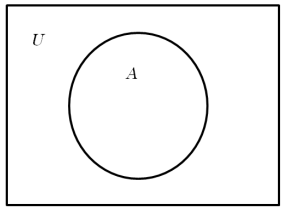
\includegraphics[scale=0.5]{5.png}
			
			\caption{一个集合$A$的文氏图}
			
		\end{figure}
		
	\end{frame}

	\begin{frame}{文氏图}
		
		当要表示多个集合时,对任意集合$A$,$B$,除非说明没有元素同时属于$A$和$B$,否则表示$A$的圆形要与表示$B$的圆形\textcolor{red}{\text{相交}}。也就是说,若要研究$n$个集合,会有$2^n$个互不重叠的封闭区间。
		
		两个圆形重叠的部分表示同时属于$A$和$B$的元素,圆形$A$中不与$B$重叠的部分表示属于$A$,不属于$B$的元素,圆形$B$中不与$A$重叠的部分表示属于$B$,不属于$A$的元素。
		
		\begin{figure}
			
			\centering
			
			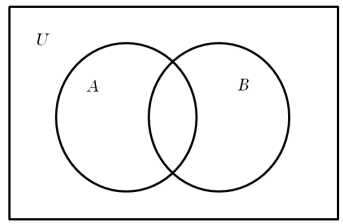
\includegraphics[scale=0.5]{0.png}
			
			\caption{两个集合$A$和$B$的文氏图}
			
		\end{figure}
		
	\end{frame}

	\begin{frame}{成员关系表}
		
		成员关系表是指用\textcolor{red}{\text{表格}}来研究集合的关系。当要研究$n$个集合时,成员关系关系表有$2^n$行,每一行对应表示$n$个集合的文氏图一个互不重叠的封闭区域。前$n$列对应$n$个集合,其余列表示集合表达式如$S$等。
		
		\begin{table}
			
			\centering
			
			\caption{有三个集合$A$,$B$,$C$的成员关系表}
			
			\begin{tabular}{|c|c|c|c|c|}
				\hline
				$A$ & $B$ & $C$ & $\dots$ & $S$\\
				\hline
				0 & 0 & 0 &  & 0\\
				\hline
				0 & 0 & 1 &  & 0\\
				\hline
				0 & 1 & 0 &  & 0\\
				\hline
				0 & 1 & 1 &  & 0\\
				\hline
				1 & 0 & 0 &  & 0\\
				\hline
				1 & 0 & 1 &  & 0\\
				\hline
				1 & 1 & 0 &  & 1\\
				\hline
				1 & 1 & 1 &  & 0\\
				\hline
			\end{tabular}
		
		\end{table}
		
	\end{frame}

	\section{习题讲解}
	
	\begin{frame}{使用元素枚举法和性质概括法定义下面集合}
		
		\begin{itemize}
			
			\item<1>1到100中17的倍数构成的集合
			
			\begin{itemize}
				
				\item<1>\textcolor{red}{\text{元素枚举法}}:$\{17,34,51,68,85\}$
				
				\item<1>\textcolor{red}{\text{性质概况法}}:$\{17k|k\in N\wedge 1<17k<100\}$。
				
			\end{itemize}
			
			
			\item<1>长度为4且含有偶数个1的二进制串构成的集合
			
			\begin{itemize}
				
				\item<1>\textcolor{red}{\text{元素枚举法}}:$\{0000,0011,0101,0110,1001,1010,1100,1111\}$
				
				\item<1>\textcolor{red}{\text{性质概况法}}:$\{w|w\in E^{*}\text{且}w\text{的长度为4且有偶数个}1\}$,$E=\text{字母集}\{0,1\}$,$E^{*}\text{表示字母集}E\text{构成的所有集合}$。
				
			\end{itemize}
			
			
		\end{itemize}
	
		\textcolor{mymauve}{元素枚举法只需要列出所有元素即可,性质概括法重点在于找到元素之间的共同性质。}
				
	\end{frame}
	
	\begin{frame}{使用归纳法定义正奇数数集$O$}
		
		\begin{itemize}
			
			\item<1>归纳基:$1\in O$
			
			\item<1>归纳步:如果正整数$n$属于$O$,则$n+2$属于$O$
			
			\item<1>最小化:集合$O$的每个元素要么是由归纳基给出的基本元素,要么是由基本元素通过有限次归纳步得到
			
		\end{itemize}
		
		\textcolor{mymauve}{最小化对所有归纳定义都是一样的,可以省略。在做出归纳定义时,我们需要找到所谓的基本元素,通过这些元素和一定的规则(归纳步),我们可以构建其集合的所有元素,不漏不多。}
		
	\end{frame}

	\begin{frame}{判断公式的真值}
		
		$$A=\{x+y|x,y\in N,1\leqslant x\leqslant 4,1\leqslant y^2\leqslant 10\}$$
		
		\begin{itemize}
			
			\item<1>$\forall x(x\in A\leftrightarrow\exists y\exists z(1\leqslant y\leqslant 4\wedge1\leqslant z^2\leqslant10\wedge x=y+z))$
			
			$\text{真值为1,其实}\forall x(x\in A\leftrightarrow\exists y\exists z(1\leqslant y\geqslant 4\wedge1\leqslant z^2\leqslant10\wedge x=y+z))$就是$A$的定义,与公式相比,只是替换了名字罢了。
			
			\item<1>$\forall x\forall y((x+y)\in A\rightarrow (1\leqslant x\leqslant 4\wedge 1\leqslant y^2\leqslant 10))$
			
			真值为0,只要举出反例即可证明,比如当$x=1$,$y=6$时,$x+y=7\in A$,但$y^2\geqslant 10$。
			
		\end{itemize}
		
		\textcolor{mymauve}{判断真值为0,只需要举出反例。判断真值为1,需要运用逻辑公式中真值判断的知识。}
		
	\end{frame}
	
	\section{总结}
	
	\begin{frame}{总结}
		
		\begin{itemize}
			
			\item<1>集合的定义
			\begin{itemize}
	
				\item<1>元素枚举法
				
				\item<1>性质概括法
				
				\item<1>归纳定义法
				
			\end{itemize}
		
			\item<1>集合之间的关系
			\begin{itemize}
				
				\item<1>子集
				
				\item<1>相等
				
				\item<1>真子集
				
			\end{itemize}	
		
			\item<1>集合的表示
			\begin{itemize}
				
				\item<1>文氏图
				
				\item<1>成员关系表
				
			\end{itemize}
			
		\end{itemize}
	\end{frame}
	
	\begin{frame}{Thank you}
		\begin{center}
			\begin{minipage}{\textwidth}
				\setbeamercolor{mybox}{fg=white, bg=black!50!blue}
				\begin{beamercolorbox}[wd=0.70\textwidth, rounded=true, shadow=true]{mybox}
					\LARGE \centering Thank you for listening!  %结束语
				\end{beamercolorbox}
			\end{minipage}
		\end{center}
	\end{frame}
	
	
	% -----------------------------------------------------------------------------
\end{document}
%文档结束
